\documentclass[aspectratio=169]{beamer}
\usepackage[T1]{fontenc}
\usepackage{lmodern}
\usepackage{tikz}
\usepackage{xcolor}
\usetikzlibrary{positioning, arrows.meta, shapes.geometric, shapes.misc, fit, calc, backgrounds}
\usetheme{metropolis}
\usefonttheme{professionalfonts}
\setbeamertemplate{footline}{}
\setbeamertemplate{navigation symbols}{}
\setbeamerfont{frametitle}{size=\large}

\definecolor{BlueA}{HTML}{174A7E}
\definecolor{BlueB}{HTML}{E4F0FB}
\definecolor{GreenA}{HTML}{2D7D46}
\definecolor{GreenB}{HTML}{E4F5E7}
\definecolor{OrangeA}{HTML}{B46A1E}
\definecolor{OrangeB}{HTML}{FAEBD7}
\definecolor{GrayA}{HTML}{59636E}
\definecolor{GrayB}{HTML}{EEF2F5}
\definecolor{PurpleA}{HTML}{5B4B8A}
\definecolor{PurpleB}{HTML}{EEEAF8}
\definecolor{TealA}{HTML}{2A7E7E}
\definecolor{TealB}{HTML}{E0F2F2}
\definecolor{RedA}{HTML}{A93433}

\tikzset{
  box/.style={draw, rounded corners=2.5pt, align=center,
              font=\scriptsize, minimum height=1.05cm,
              inner sep=4.5pt, thick},
  frame/.style={fill=PurpleB, draw=PurpleA},
  hyp/.style={fill=BlueB, draw=BlueA},
  plan/.style={fill=GreenB, draw=GreenA},
  envb/.style={fill=GrayB, draw=GrayA},
  refl/.style={fill=OrangeB, draw=OrangeA},
  store/.style={fill=TealB, draw=TealA},
  skl/.style={fill=GreenB, draw=GreenA, dashed},
  arr/.style={-{Latex[length=1.6mm]}, thick},
  arrdash/.style={-{Latex[length=1.6mm]}, thick, dashed, draw=GrayA},
  badge/.style={draw=RedA, fill=white, rounded corners=2pt,
                font=\tiny\bfseries, inner sep=2pt, text=RedA}
}

\newcommand{\code}[1]{\texttt{\scriptsize #1}}

\begin{document}

\begin{frame}{Per-turn loop --- v52 (M1--M4 + image + SKILL.md, no leak)}
\centering
\resizebox{0.97\textwidth}{!}{%
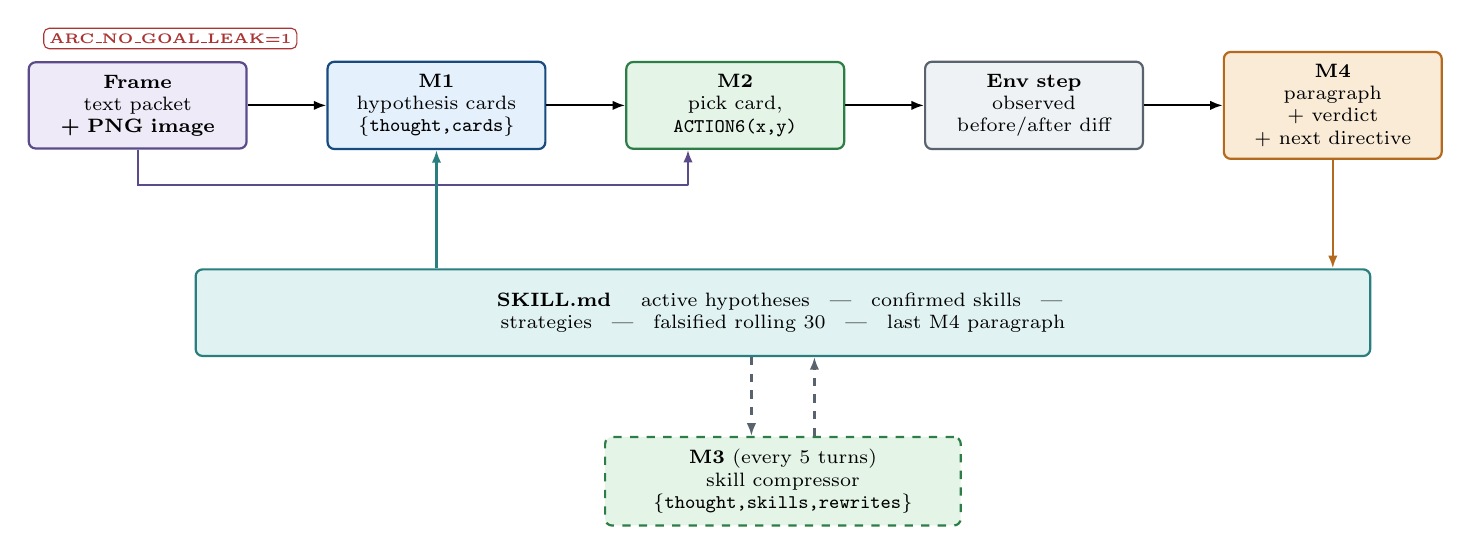
\begin{tikzpicture}[node distance=0.85cm and 1.0cm]

  % ----- Top row: per-turn pipeline -----
  \node[box, frame, text width=2.45cm] (frame)
    {\textbf{Frame}\\text packet\\\textbf{+ PNG image}};

  \node[box, hyp, right=of frame, text width=2.45cm] (m1)
    {\textbf{M1}\\hypothesis cards\\\code{\{thought,cards\}}};

  \node[box, plan, right=of m1, text width=2.45cm] (m2)
    {\textbf{M2}\\pick card,\\\code{ACTION6(x,y)}};

  \node[box, envb, right=of m2, text width=2.45cm] (env)
    {\textbf{Env step}\\observed\\before/after diff};

  \node[box, refl, right=of env, text width=2.45cm] (m4)
    {\textbf{M4}\\paragraph + verdict\\+ next directive};

  % ----- SKILL.md spans full width -----
  \node[box, store, below=1.5cm of m1.south,
        xshift=4.4cm, text width=14.6cm, minimum height=1.1cm] (skill)
    {\textbf{SKILL.md} \quad active hypotheses \;\;|\;\; confirmed skills \;\;|\;\;
     strategies \;\;|\;\; falsified rolling 30 \;\;|\;\; last M4 paragraph};

  % ----- M3 below, dashed (every 5 turns) -----
  \node[box, skl, below=1.0cm of skill.south,
        text width=4.2cm] (m3)
    {\textbf{M3} \scriptsize(every 5 turns)\\skill compressor\\\code{\{thought,skills,rewrites\}}};

  % ----- Top-row pipeline arrows -----
  \draw[arr] (frame.east) -- (m1.west);
  \draw[arr] (m1.east) -- (m2.west);
  \draw[arr] (m2.east) -- (env.west);
  \draw[arr] (env.east) -- (m4.west);

  % ----- Image side-feed: Frame also feeds M2 with image -----
  \draw[arr, draw=PurpleA]
    (frame.south) |- ($(frame.south) + (0,-0.45)$) -|
    ($(m2.south) + (-0.6,-0.45)$) -- ($(m2.south) + (-0.6,0)$);

  % ----- M4 -> SKILL.md (write paragraph + falsified entries) -----
  \draw[arr, draw=OrangeA] (m4.south) -- (m4.south |- skill.north);

  % ----- SKILL.md -> M1 (read slice + directive) -----
  \draw[arr, draw=TealA]
    (skill.north -| m1.south) -- (m1.south);

  % ----- M3 <-> SKILL.md (read recent obs, write skills+rewrites) -----
  % Two parallel dashed arrows side-by-side: down = read, up = write.
  \draw[arrdash] ($(skill.south) + (-0.4,0)$) -- ($(m3.north) + (-0.4,0)$);
  \draw[arrdash] ($(m3.north) + (0.4,0)$) -- ($(skill.south) + (0.4,0)$);

  % ----- NO-LEAK gate badge (kept inside frame's column) -----
  \node[badge, above right=0.15cm and -1.2cm of frame.north]
    (badge) {ARC\_NO\_GOAL\_LEAK=1};

\end{tikzpicture}%
}

\vspace{0.5em}
\centering
\footnotesize
M1+M2 see grid as image \emph{and} text; M4 closes the loop with paragraph
reasoning into SKILL.md; M3 compresses every 5 turns.
\end{frame}

\end{document}
